\PassOptionsToPackage{unicode=true}{hyperref} % options for packages loaded elsewhere
\PassOptionsToPackage{hyphens}{url}
%
\documentclass[]{article}
\usepackage{lmodern}
\usepackage{amssymb,amsmath}
\usepackage{ifxetex,ifluatex}
\usepackage{fixltx2e} % provides \textsubscript
\ifnum 0\ifxetex 1\fi\ifluatex 1\fi=0 % if pdftex
  \usepackage[T1]{fontenc}
  \usepackage[utf8]{inputenc}
  \usepackage{textcomp} % provides euro and other symbols
\else % if luatex or xelatex
  \usepackage{unicode-math}
  \defaultfontfeatures{Ligatures=TeX,Scale=MatchLowercase}
\fi
% use upquote if available, for straight quotes in verbatim environments
\IfFileExists{upquote.sty}{\usepackage{upquote}}{}
% use microtype if available
\IfFileExists{microtype.sty}{%
\usepackage[]{microtype}
\UseMicrotypeSet[protrusion]{basicmath} % disable protrusion for tt fonts
}{}
\IfFileExists{parskip.sty}{%
\usepackage{parskip}
}{% else
\setlength{\parindent}{0pt}
\setlength{\parskip}{6pt plus 2pt minus 1pt}
}
\usepackage{hyperref}
\hypersetup{
            pdfborder={0 0 0},
            breaklinks=true}
\urlstyle{same}  % don't use monospace font for urls
\usepackage[margin=2cm]{geometry}
\usepackage{graphicx,grffile}
\makeatletter
\def\maxwidth{\ifdim\Gin@nat@width>\linewidth\linewidth\else\Gin@nat@width\fi}
\def\maxheight{\ifdim\Gin@nat@height>\textheight\textheight\else\Gin@nat@height\fi}
\makeatother
% Scale images if necessary, so that they will not overflow the page
% margins by default, and it is still possible to overwrite the defaults
% using explicit options in \includegraphics[width, height, ...]{}
\setkeys{Gin}{width=\maxwidth,height=\maxheight,keepaspectratio}
\setlength{\emergencystretch}{3em}  % prevent overfull lines
\providecommand{\tightlist}{%
  \setlength{\itemsep}{0pt}\setlength{\parskip}{0pt}}
\setcounter{secnumdepth}{0}
% Redefines (sub)paragraphs to behave more like sections
\ifx\paragraph\undefined\else
\let\oldparagraph\paragraph
\renewcommand{\paragraph}[1]{\oldparagraph{#1}\mbox{}}
\fi
\ifx\subparagraph\undefined\else
\let\oldsubparagraph\subparagraph
\renewcommand{\subparagraph}[1]{\oldsubparagraph{#1}\mbox{}}
\fi

% set default figure placement to htbp
\makeatletter
\def\fps@figure{htbp}
\makeatother


\date{}

\begin{document}

\hypertarget{introduction}{%
\section{Introduction}\label{introduction}}

\href{https://www.youtube.com/watch?v=IUk9o9wvX1Y\&t=3094s}{\textbf{{[}LINK{]}}:
Entire lecture on youtube\textsuperscript{1}}

Need more main memory (capacity)

\begin{itemize}
\tightlist
\item
  Modern application are (increasingly) data-intensive
\item
  Many applications share main memory

  \begin{itemize}
  \tightlist
  \item
    Cloud computing
  \item
    Many-core CPUs
  \end{itemize}
\end{itemize}

\hypertarget{major-trends-affecting-main-memory}{%
\subsection{Major Trends Affecting Main
Memory}\label{major-trends-affecting-main-memory}}

\begin{enumerate}
\def\labelenumi{\arabic{enumi}.}
\tightlist
\item
  Need for main memory capacity, bandwidth, QoS increasing

  \begin{itemize}
  \tightlist
  \item
    Multi-core: increasing number of cores
  \item
    Data intensive applications: increasing demand/hunger for data
  \item
    Consolidation: cloud computing, GPUs, mobile
  \end{itemize}
\item
  Main memory energy/power is a key system design concern

  \begin{itemize}
  \tightlist
  \item
    DRAM consumes more power when idle and needs periodic refresh
  \end{itemize}
\item
  DRAM technology scaling is ending

  \begin{itemize}
  \tightlist
  \item
    DRAM will not scale easily below X nm
  \item
    Scaling has provided many benefits

    \begin{itemize}
    \tightlist
    \item
      higher capacity, higher density, lower cost, lower energy
    \end{itemize}
  \end{itemize}
\end{enumerate}

\hypertarget{dram-scaling-problem}{%
\subsection{DRAM Scaling Problem}\label{dram-scaling-problem}}

DRAM stores charge in a capacitor (charge-based memory)

\begin{itemize}
\tightlist
\item
  Capacitor must be large enough for reliable sensing
\item
  DRAM hard to scale
\end{itemize}

Evidence of Scaling Problem (\textbf{Row Hammer})

\begin{itemize}
\tightlist
\item
  DRAM uses low and high voltage to insert data into a cell
\item
  Repeatedly opening and closing a row enough times within a refresh
  interval induces disturbance errors in adjacent rows in most real DRAM
  chips bought today.

  \begin{itemize}
  \tightlist
  \item
    Aggressor Row (causing disturbance)
  \end{itemize}
\item
  Experiment shows 80\% of DRAMs are effected by this issue
\end{itemize}

\begin{figure}
\centering
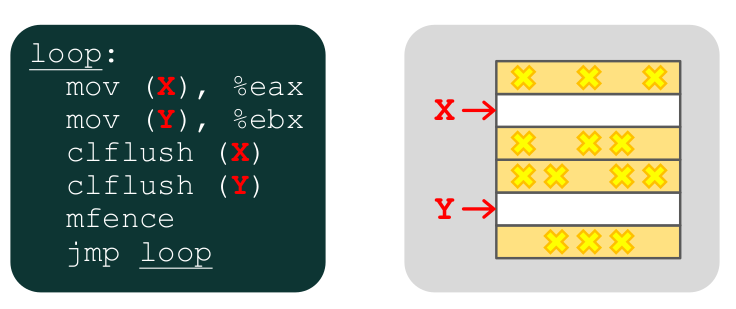
\includegraphics[width=0.8\textwidth,height=\textheight]{./tex2pdf.-ee748c56ff17e1e1/8b1c1a0d77db887c14f21bd20d64b4f7d321df1c.png}
\caption{Example of rowhammer attack in DRAM}
\end{figure}

\begin{itemize}
\tightlist
\item
  mov = Load x into eax register
\item
  clflush = Flush register
\item
  mfence = Ensure that memory instructions actually occur
\item
  jmp = Branch jump to beginning of loop
\end{itemize}

\hypertarget{security-implications}{%
\subsubsection{Security Implications}\label{security-implications}}

\begin{itemize}
\tightlist
\item
  Memory isolation: an access to one address memory should not have
  unintended side effects on data stored in other addresses.
\item
  Rowhammer is a problem with recent DRAM devices (as of 2010)
\item
  Can use rowhammer to induce bit flips to gain kernel privileges on
  x86-64 when ran as unprivileged userland process.
\item
  Rowhammer can induce bit flips in page table entries
\item
  Able too gain access to its own page table, and hence gain read-write
  access to all of physical memory
\end{itemize}

\hypertarget{main-memory-in-the-system}{%
\subsection{Main Memory in the System}\label{main-memory-in-the-system}}

Physical address space:

\begin{itemize}
\tightlist
\item
  Maximum size of main memory: total number of uniquely identifiable
  locations
\end{itemize}

Physical addressability

\begin{itemize}
\tightlist
\item
  Minimum size of data in memory can be addressed
\item
  Byte-addressable, word-addressable, 64-bit-addressable
\item
  Microarchitectural addressability depends on the abstraction level of
  the implementation
\end{itemize}

\newpage

\hypertarget{dram-subsystem-bottom-up}{%
\section{DRAM Subsystem (Bottom Up)}\label{dram-subsystem-bottom-up}}

Abstract Diagram:

\begin{itemize}
\tightlist
\item
  Channel (Highest in abstraction)
\item
  Due Inline Memory Module (DIMM)
\item
  Rank
\item
  Chip
\item
  Bank
\item
  Row/Column
\end{itemize}

\hypertarget{dram-memory-bank-organization}{%
\subsection{DRAM Memory Bank
Organization}\label{dram-memory-bank-organization}}

\begin{figure}
\centering
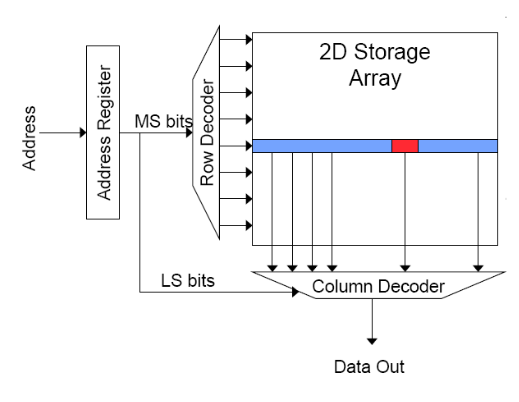
\includegraphics[width=0.6\textwidth,height=\textheight]{./tex2pdf.-ee748c56ff17e1e1/8dd461ecda617c9c6e95771cb49d649644087cc6.png}
\caption{Example of a Memory Bank}
\end{figure}

Read access sequence:

\begin{enumerate}
\def\labelenumi{\arabic{enumi}.}
\tightlist
\item
  Decode row address
\item
  Read entire row
\item
  Amplify row data
\item
  Decode column address and select subset of row (send to output)
\item
  Precharge bit lines (WTF LOL)
\end{enumerate}

\hypertarget{interleaving-banking}{%
\subsubsection{Interleaving (Banking)}\label{interleaving-banking}}

Problem: a single monolithic memory array takes long to access and does
not enable multiple access in parallel (high cost).

Goal: reduce the latency of memory array access and enable multiple
access in parallel

Idea: divide the array into multiple banks that can be accessed
independently (in the same cycle or in consecutive cycles)

\begin{itemize}
\tightlist
\item
  Each bank is smaller than the entire memory storage
\item
  Accesses to different banks can be overlapped
\end{itemize}

Key Issue: How to map data to different banks?

\hypertarget{page-mode-dram}{%
\subsubsection{Page Mode DRAM}\label{page-mode-dram}}

\begin{itemize}
\tightlist
\item
  A DRAM bank is a 2D array of cells: rows x columns
\item
  A DRAM row is also called a DRAM page
\item
  The activated row is placed in a row buffer
\item
  Each address is a \textless{}row, column\textgreater{} pair
\item
  Access to a closed row:

  \begin{itemize}
  \tightlist
  \item
    Activate command opens row (placed into row buffer)
  \item
    Read/write command reads/write column in the row buffer
  \item
    Precharge command closes the row and prepares the bank for next
    access
  \end{itemize}
\item
  Access to an open row:

  \begin{itemize}
  \tightlist
  \item
    No need for activate command
  \end{itemize}
\end{itemize}

\begin{figure}
\centering
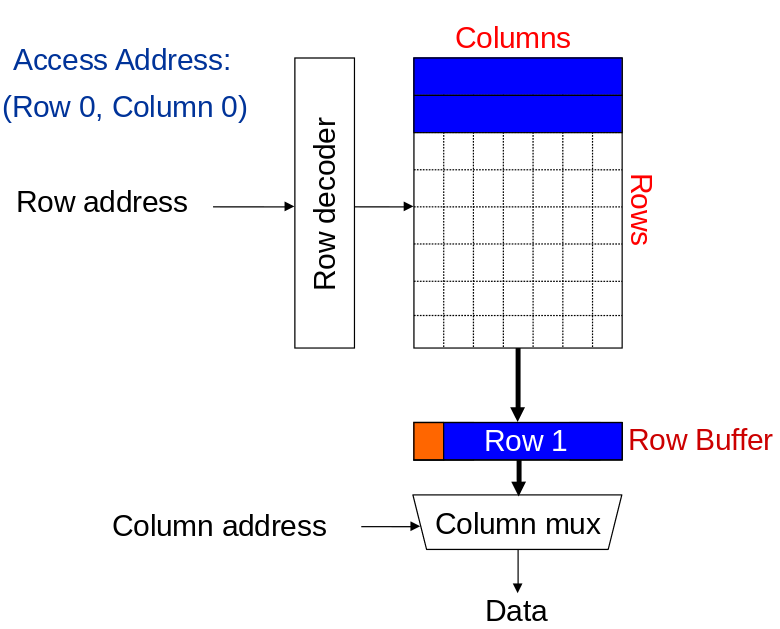
\includegraphics[width=0.7\textwidth,height=\textheight]{./tex2pdf.-ee748c56ff17e1e1/7a56a62ac4e4deef8daeba0fa22e2d01d01b5943.png}
\caption{Example of DRAM Bank operation}
\end{figure}

Explanation of DRAM bank operation:

\begin{itemize}
\tightlist
\item
  Accessing address (Row 0, Col 0)

  \begin{itemize}
  \tightlist
  \item
    Row address gets sent to row decoder and retrieve the respective row
    and puts it in the row buffer
  \item
    The column address is sent to column mux which extracts the data
    from the column in the row buffer and sends it to the user as the
    data
  \end{itemize}
\item
  Accessing address (Row 0, Col 69) assuming you just accessed (Row 0,
  Col 0)

  \begin{itemize}
  \tightlist
  \item
    You will get a hit in the row decoder and therefore only need to do
    the column mux part to get the 69\textsuperscript{th} column of data
  \end{itemize}
\item
  Accessing address (Row 1, Col 0) assuming you just accessed (Row 0,
  Col 69)

  \begin{itemize}
  \tightlist
  \item
    Miss, gotta do both again
  \end{itemize}
\end{itemize}

\hypertarget{dram-chips}{%
\subsection{DRAM Chips}\label{dram-chips}}

Consists of multiple banks (2-16 in DRAM)

Banks share command/address/data buses

The chip itself has a narrow interface (4-16 bits per read)

\hypertarget{dram-rank-and-module}{%
\subsection{DRAM Rank and Module}\label{dram-rank-and-module}}

Rank: multiple chips operated together to form a wide interface

\begin{itemize}
\tightlist
\item
  All chips comprising a rank are controlled at the same time

  \begin{itemize}
  \tightlist
  \item
    Respond to a single command
  \item
    Share address and command buses, but provide different idea
  \end{itemize}
\end{itemize}

DRAM Module: consists of one or more ranks

\begin{itemize}
\tightlist
\item
  DIMM (dual inline memory module)
\item
  This is what you plug into your motherboard
\end{itemize}

If we have chips with 8-bit interface, to read 8 bytes in a single
access, use 8 chips in a DIMM

\begin{figure}
\centering
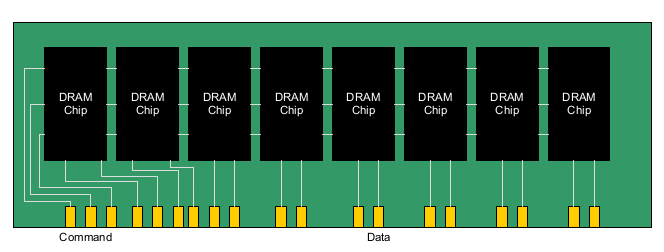
\includegraphics[width=0.6\textwidth,height=\textheight]{./tex2pdf.-ee748c56ff17e1e1/beea6dee16691a185c8dfbb616aa9effabce9a48.png}
\caption{A 64-bit wide DIMM (one rank)}
\end{figure}

\hypertarget{multiple-dimms}{%
\subsubsection{Multiple DIMMs}\label{multiple-dimms}}

Advantages: enables higher capacity

Disadvantages: interconnect complexity and energy consumption can be
high

\hypertarget{dram-channels}{%
\subsection{DRAM Channels}\label{dram-channels}}

What controls the set of DIMMs.

2 Independent Channels: 2 memory controllers

\begin{figure}
\centering
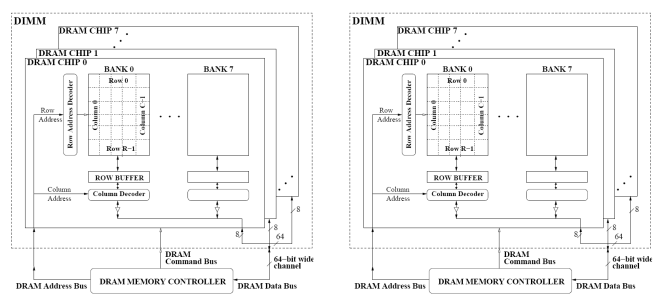
\includegraphics[width=0.9\textwidth,height=\textheight]{./tex2pdf.-ee748c56ff17e1e1/722152b1cbbf12340c2ad3f47168800019155bee.png}
\caption{Diagram of 2 memory controllers}
\end{figure}

\hypertarget{general-memory-structure}{%
\section{General Memory Structure}\label{general-memory-structure}}

\begin{figure}
\centering
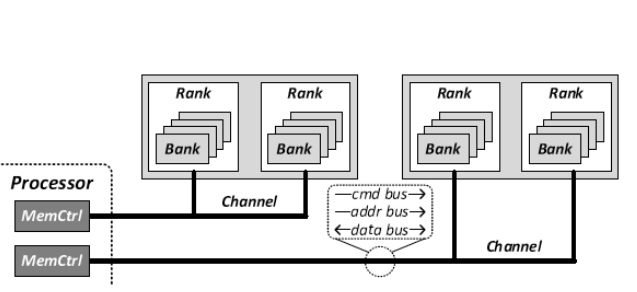
\includegraphics{./tex2pdf.-ee748c56ff17e1e1/f97cc899e87e6e510f7ed5664052ddd0c66f5bfa.png}
\caption{General memory structure}
\end{figure}

Processor send request to Channel

\begin{itemize}
\tightlist
\item
  Channel holds two DIMMs
\end{itemize}

DIMM have multiple ranks

\begin{itemize}
\tightlist
\item
  There is a front and a back each is a rank
\item
  Total of 2 ranks
\end{itemize}

Rank consist of chips

\begin{itemize}
\tightlist
\item
  Shared data bus, there is a penalty from switching one rank to another
\end{itemize}

Chip consist of multiple banks

\begin{itemize}
\tightlist
\item
  Can multiplex data to different banks
\end{itemize}

Banks has the 2D array

\newpage

\hypertarget{how-processors-gets-data-from-main-memory}{%
\subsection{How Processors Gets Data from Main
Memory}\label{how-processors-gets-data-from-main-memory}}

\begin{figure}
\centering
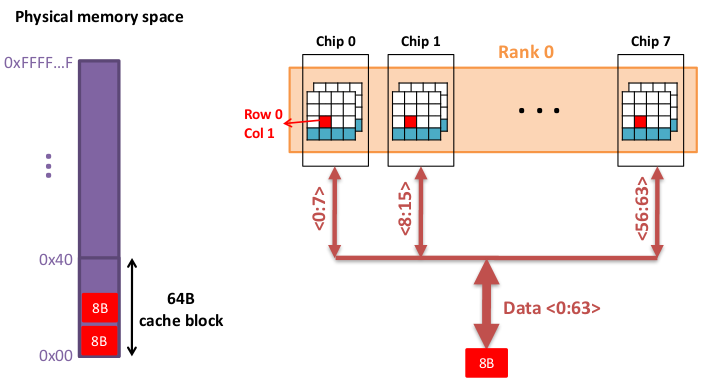
\includegraphics{./tex2pdf.-ee748c56ff17e1e1/cf36d48e85675d52cd1dcea1a7a7e327b41f1859.png}
\caption{Example: Transferring a cache block}
\end{figure}

\begin{itemize}
\tightlist
\item
  Given the 64B cache block in main memory, it gets mapped to a single
  rank
\item
  Chip (tiny square) holds 8 bits of data

  \begin{itemize}
  \tightlist
  \item
    Accessing an entire row gives you 64 bits
  \item
    With 8 chips this gives us the whole entire 64 byte representation
  \end{itemize}
\item
  A 64B cache block takes 8 I/O cycles to transfer
\item
  During the process, 8 columns are read sequentially (WE CAN PIPE LINE
  THO)
\end{itemize}

\hypertarget{multiple-banks}{%
\subsection{Multiple Banks}\label{multiple-banks}}

Multiple Banks

\begin{itemize}
\tightlist
\item
  Enable concurrent DRAM access
\item
  Multiple independent channels serve the same purpose

  \begin{itemize}
  \tightlist
  \item
    They are even better because they have separate data buses
  \item
    Increase bus bandwidth
  \end{itemize}
\item
  Enabling more concurrency still requires reducing:

  \begin{itemize}
  \tightlist
  \item
    Bank conflicts
  \item
    Channel conflicts
  \end{itemize}
\item
  How to select/randomize bank/channel indices in address

  \begin{itemize}
  \tightlist
  \item
    Lower order bits have more entropy
  \item
    Randomizing hash functions
  \end{itemize}
\end{itemize}

\newpage

\hypertarget{a-modern-dram-controller}{%
\section{A Modern DRAM Controller}\label{a-modern-dram-controller}}

\begin{figure}
\centering
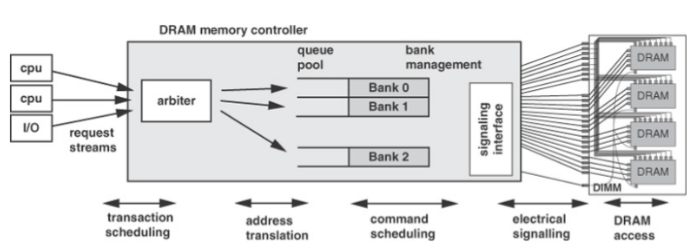
\includegraphics[width=0.85\textwidth,height=\textheight]{./tex2pdf.-ee748c56ff17e1e1/8e99ce871822a47fe3b076cbbf3a56a022e165ce.png}
\caption{Modern DRAM Controller (I)}
\end{figure}

\begin{itemize}
\tightlist
\item
  Input: request from CPU
\item
  Abiter determines where to route request
\item
  When DRAM bank not busy, controller sends one of teh queue pools into
  the DRAM
\end{itemize}

\begin{figure}
\centering
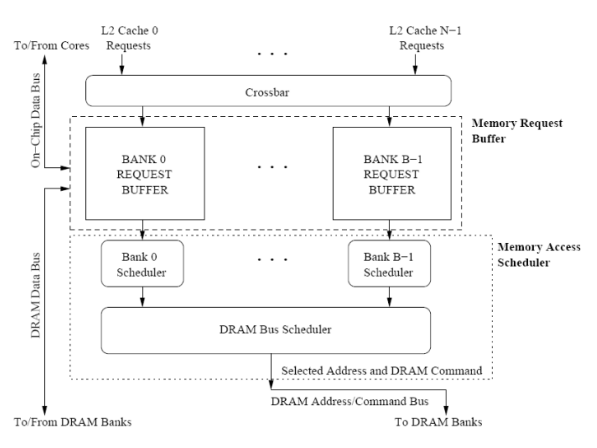
\includegraphics[width=0.8\textwidth,height=\textheight]{./tex2pdf.-ee748c56ff17e1e1/2faebcbb6c088bff74c716b76f0e7052de951bce.png}
\caption{Modern DRAM Controller (II)}
\end{figure}

\begin{itemize}
\tightlist
\item
  Request placed in buffers and then scheduled into an actually DRAM
  when not busy
\end{itemize}

\newpage

\hypertarget{dram-scheduling-policies}{%
\subsection{DRAM Scheduling Policies}\label{dram-scheduling-policies}}

First come first served (FCFS)

\begin{itemize}
\tightlist
\item
  Oldest request first
\end{itemize}

First reader, first come first served (FR-FCFS)

\begin{itemize}
\tightlist
\item
  Row-hit first
\item
  Oldest first
\item
  Goal: Maximize row buffer hit rate → maximize DRAM throughput
\end{itemize}

\hypertarget{multicore-on-chip}{%
\section{Multicore on Chip}\label{multicore-on-chip}}

\begin{figure}
\centering
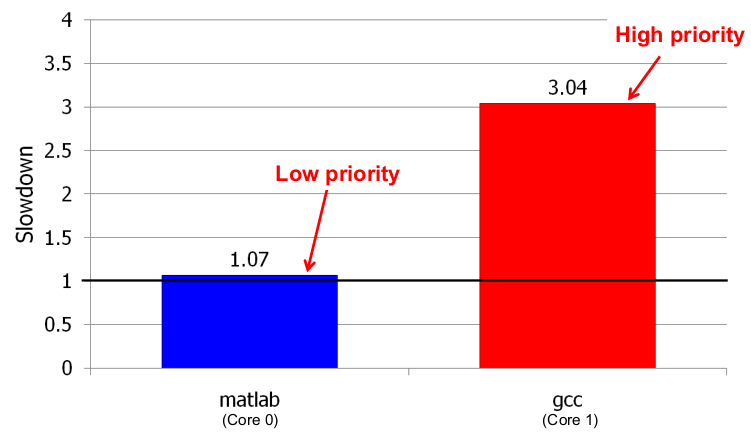
\includegraphics{./tex2pdf.-ee748c56ff17e1e1/feba0895693464b51c7c183f6d25ab611b6b5a64.png}
\caption{Unexpected Slowdowns in Multicore}
\end{figure}

We have two applications running on two different cores

\begin{itemize}
\tightlist
\item
  Expectation: no slowdown, they're running different hardware
  (different core)
\item
  Graph show otherwise, this is because they share the same DRAM system
  (main memory causing slowdown)
\item
  Even with high priority, gcc gets the slow down, why???

  \begin{itemize}
  \tightlist
  \item
    DRAM for sure, this is not because of OS resource allocation
  \end{itemize}
\item
  DRAM controller is unfair
\end{itemize}

\newpage

\hypertarget{memory-hog-oink}{%
\subsection{Memory Hog (oink)}\label{memory-hog-oink}}

\begin{figure}
\centering
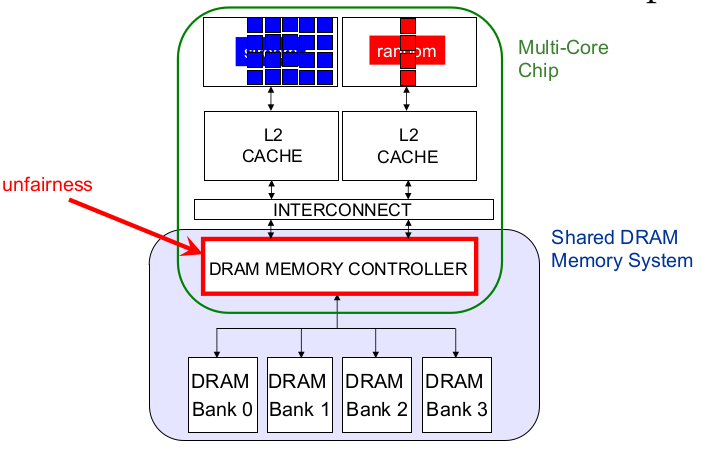
\includegraphics{./tex2pdf.-ee748c56ff17e1e1/48ee445de0deeb315ed965bd725307bae1a6bee3.png}
\caption{Example uncontrolled interference}
\end{figure}

\begin{itemize}
\tightlist
\item
  Blue = streaming application
\item
  Red = random application
\item
  Blue has better dram controlling because it access the same row
\item
  Stream application get all 4 banks first because row buffer hits
\item
  This makes it unfair for the random application (random never gets
  queued into controller) \protect\hyperlink{}{comment}: \# (add code
  implementatio of the above diagram)
\end{itemize}

\hypertarget{memory-hog-effects}{%
\subsection{Memory Hog Effects}\label{memory-hog-effects}}

Worst case scenario given a row size of 8KB and cache block size of 64B.

128 requests to a single row could be serviced before the other is
serviced

This same pattern can be seen in systems with more than 2 cores

\hypertarget{memory-hog-solution}{%
\subsection{Memory Hog Solution}\label{memory-hog-solution}}

Goal: Threads sharing main memory should experience similar slowdowns
compared to when they are run alone (fair scheduling)

\begin{itemize}
\tightlist
\item
  Also improves overall system performance by ensuring cores make
  ``proportional'' progress
\end{itemize}

Idea: Memory controller estimates each thread's slowdown due to
interference and schedules requests in a way to balance the slowdowns

Done with \textbf{Stall-time fair memory (STFM) scheduling}

\hypertarget{stall-time-fairness-in-shared-dram-systems}{%
\subsubsection{Stall-Time Fairness in Shared DRAM
Systems}\label{stall-time-fairness-in-shared-dram-systems}}

Fair DRAM System: when it equalizes the slowdown of equal priority
threads relative to their speed when ran alone

\begin{itemize}
\tightlist
\item
  DRAM-related stall-time: The time a thread spends waiting for DRAM
  memory
\end{itemize}

Memory Slowdown =
\(\displaystyle\frac{\text{ST-Shared}}{\text{ST-Alone}}\)

\begin{itemize}
\tightlist
\item
  ST-Shared: DRAM-related stall-time when the thread runs with other
  threads
\item
  ST-Alone: DRAM-related stall-time when thread runs alone
\end{itemize}

STFM scheduler aims to \textbf{equalize} memory-slowdown for interfering
threads, without sacrificing performance

\begin{itemize}
\tightlist
\item
  Consider inherent DRAM performance of each thread
\item
  Aims to allow proportional progress of threads
\end{itemize}

\hypertarget{stfm-scheduling-algorithm}{%
\subsubsection{STFM Scheduling
Algorithm}\label{stfm-scheduling-algorithm}}

For each thread, the DRAM controller

\begin{itemize}
\tightlist
\item
  Tracks ST-Shared
\item
  Estimates ST-Alone
\end{itemize}

Each cycle, the DRAM controller

\begin{itemize}
\tightlist
\item
  Computes slowdown = ST-Shared / ST-Alone for threads with legal
  requests
\item
  Computes unfairness = Max Slowdown / Min Slowdown
\end{itemize}

If unfairness \textless{} \(\alpha\)

\begin{itemize}
\tightlist
\item
  Use DRAM throughput oriented scheduling policy
\end{itemize}

If unfairness \(\ge\) \(\alpha\)

\begin{itemize}
\tightlist
\item
  Use fairness-oriented scheduling policy

  \begin{enumerate}
  \def\labelenumi{\arabic{enumi}.}
  \tightlist
  \item
    requests from thread with MAX slowdown first
  \item
    row hit first, oldest first
  \end{enumerate}
\end{itemize}

\newpage

\hypertarget{parallelism-aware-batch-scheduling-introduction}{%
\section{Parallelism-Aware Batch Scheduling:
Introduction}\label{parallelism-aware-batch-scheduling-introduction}}

\hypertarget{another-problem-due-to-interference}{%
\subsection{Another Problem Due to
Interference}\label{another-problem-due-to-interference}}

Processors try to tolerate the latency of DRAM requests by generating
multiple outstanding requests

\begin{itemize}
\tightlist
\item
  Memory-Level Parallelism (MLP)
\item
  Out-of-order execution, non-block caches, runahead execution
\end{itemize}

Effective only if the DRAM controller actually services the multiple
requests in parallel in DRAM banks

Multiple threads share the DRAM controller

DRAM controllers are not aware of a thread's MLP

\begin{itemize}
\tightlist
\item
  Can service each thread's outstanding requests serially, not in
  parallel
\end{itemize}

\hypertarget{bank-parallelism-example}{%
\subsection{Bank Parallelism Example}\label{bank-parallelism-example}}

\begin{figure}
\centering
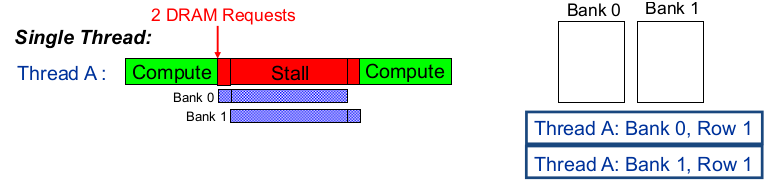
\includegraphics{./tex2pdf.-ee748c56ff17e1e1/ada8ab1ceade888491eb9d14db3d6690d9805ce3.png}
\caption{Bank Parallelism}
\end{figure}

\begin{itemize}
\tightlist
\item
  Bank access latencies of the two requests are overlapped
\item
  Thread stalls for ONE bank access latency
\item
  Parallelism good
\end{itemize}

\hypertarget{bank-parallelism-interference-example}{%
\subsection{Bank Parallelism Interference
Example}\label{bank-parallelism-interference-example}}

\begin{figure}
\centering
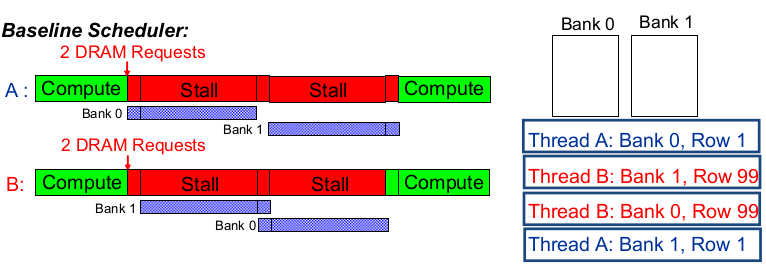
\includegraphics{./tex2pdf.-ee748c56ff17e1e1/96b8b201dd49a234602d2f78ce076a74c561fa84.png}
\caption{Bank Parallelism Interference}
\end{figure}

\begin{itemize}
\tightlist
\item
  Bank access latencies of each thread serialized
\item
  Each thread stalls for TWO bank access latencies
\item
  Between the two threads the executions are parallelized, but you still
  have two stalls
\item
  Handles thread by order in which they appear
\end{itemize}

\hypertarget{parallelism-aware-scheduler-example}{%
\subsection{Parallelism-Aware Scheduler
Example}\label{parallelism-aware-scheduler-example}}

\begin{figure}
\centering
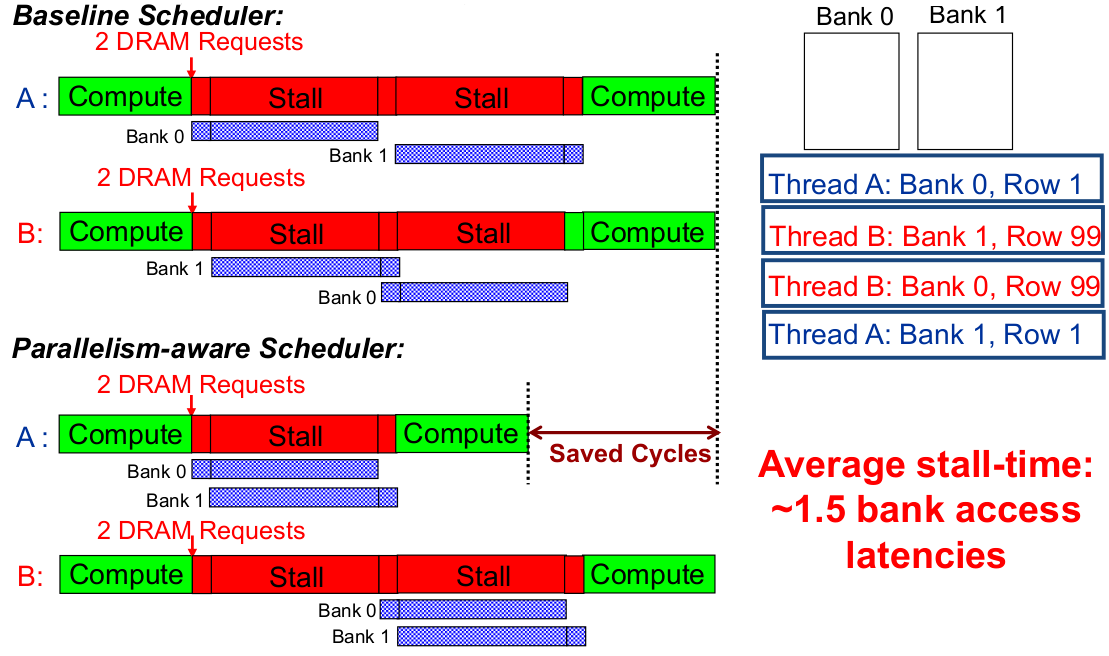
\includegraphics{./tex2pdf.-ee748c56ff17e1e1/a1d93c4ff3a8fa9c059a7a258f6fde35ebaef550.png}
\caption{Solution: Parallelism-Aware Batch Scheduling}
\end{figure}

\begin{itemize}
\tightlist
\item
  Instead of doing it by order, it recognizes parallelism and will
  execute A's request in parallel
\item
  This save \emph{average} stall time because A has save cycles
\end{itemize}

\hypertarget{parallelism-aware-batch-scheduling-par-bs}{%
\section{Parallelism-Aware Batch Scheduling
(PAR-BS)}\label{parallelism-aware-batch-scheduling-par-bs}}

Principle 1: Parallelism-awareness

\begin{itemize}
\tightlist
\item
  Schedule requests from a thread (to different banks) back to back

  \begin{itemize}
  \tightlist
  \item
    Preserves each thread's bank parallelism
  \item
    Can cause starvation
  \end{itemize}
\end{itemize}

Principle 2: Request Batching

\begin{itemize}
\tightlist
\item
  Group a fixed number of oldest requests from each thread into a
  ``batch''
\item
  Service the batch before all other requests

  \begin{itemize}
  \tightlist
  \item
    Form a new batch when the current one is done
  \item
    Eliminates starvation, provides fairness
  \item
    Allows parallelism-awareness within a batch
  \end{itemize}
\end{itemize}

\hypertarget{par-bs-components}{%
\subsection{PAR-BS Components}\label{par-bs-components}}

Two components:

\begin{enumerate}
\def\labelenumi{\arabic{enumi}.}
\tightlist
\item
  Request batching
\item
  Within-batch scheduling
\end{enumerate}

\hypertarget{request-batching}{%
\subsubsection{Request Batching}\label{request-batching}}

Each memory request has a bit (marked) associated with it

Batch formation:

\begin{itemize}
\tightlist
\item
  Mark up to Marking-Cap oldest requests per bank for each thread
\item
  Marked requests constitute the batch
\item
  Form a new batch when no marked requests are left
\end{itemize}

Marked requests are prioritized over unmarked ones

\begin{itemize}
\tightlist
\item
  No reordering of requests across batches: no starvation, high fairness
\end{itemize}

How to prioritize requests within branch?

\begin{itemize}
\tightlist
\item
  WITHIN BATCH SCHEDULING
\end{itemize}

\hypertarget{within-batch-scheduling}{%
\subsubsection{Within-Batch Scheduling}\label{within-batch-scheduling}}

Can use any DRAM scheduling policy

\begin{itemize}
\tightlist
\item
  FR-FCFS (row hit first, then oldest first) exploits row-buffer
  locality
\end{itemize}

But, we also want to preserve intra-thread bank parallelism

\begin{itemize}
\tightlist
\item
  Service each thread's requests back to back
\item
  How???
\end{itemize}

How: Scheduler computes a ranking of threads when the batch is formed

\begin{itemize}
\tightlist
\item
  Higher-ranked threads are prioritized over lower-ranked ones
\item
  Improves likelihood that requests from a thread are serviced in
  parallel by different banks

  \begin{itemize}
  \tightlist
  \item
    Different threads prioritized in the same order across all banks
  \end{itemize}
\end{itemize}

\hypertarget{how-to-rank-threads-within-a-batch}{%
\subsection{How to Rank Threads within a
Batch}\label{how-to-rank-threads-within-a-batch}}

Ranking scheme affects system throughput and fairness

Goals I: Maximize system throughput

\begin{itemize}
\tightlist
\item
  Minimize average stall-time of threads within the batch
\end{itemize}

Goal II: Minimize unfairness (Equalize the slowdown of threads)

\begin{itemize}
\tightlist
\item
  Service threads with inherently low stall-time early in the batch
\item
  Insight: delaying memory non-intensive threads results in high
  slowdown
\end{itemize}

Shortest stall-time first (shortest job first) ranking

\begin{itemize}
\tightlist
\item
  Provides optimal system throughput
\item
  Controller estimates each thread's stall-time within the batch
\item
  Ranks threads with shorter stall-time higher
\end{itemize}

\hypertarget{shortest-stall-time-first-ranking}{%
\subsection{Shortest Stall-Time First
Ranking}\label{shortest-stall-time-first-ranking}}

Maximum number of marked requests to any bank (max-bank-load)

\begin{itemize}
\tightlist
\item
  Ranked thread with lower max-bank-load higher (\textasciitilde{}low
  stall-time)
\end{itemize}

Total number of marked requests (total-load)

\begin{itemize}
\tightlist
\item
  Break ties: ranked thread with lower total-load higher
\end{itemize}

\hypertarget{example}{%
\subsubsection{Example}\label{example}}

\hypertarget{hardware-costs}{%
\subsubsection{Hardware Costs}\label{hardware-costs}}

\textless{} 1.5KB storage cost for:

\begin{itemize}
\tightlist
\item
  8-core system with 128-entry memory request buffer
\end{itemize}

No complex operations (division)

Not on the critical path

\begin{itemize}
\tightlist
\item
  Scheduler makes a decision only every DRAM cycle
\end{itemize}

\end{document}
